\documentclass{beamer}

\usepackage{helvet}
\usepackage{hyperref, graphicx}
\usepackage{amsthm}
\usepackage{etoolbox}
\usepackage{multicol}

\usetheme[progressbar=frametitle, numbering=none]{metropolis}
\usecolortheme[snowy]{owl}
\setbeamertemplate{navigation symbols}{}
\AtBeginSection[ ]
{
\begin{frame}{Outline}
    \tableofcontents[currentsection]
\end{frame}
}

% Default fixed font does not support bold face
\DeclareFixedFont{\ttb}{T1}{txtt}{bx}{n}{11} % for bold
\DeclareFixedFont{\ttm}{T1}{txtt}{m}{n}{12}  % for normal - use in headings

% Custom colors
\usepackage{color}
\definecolor{TUGray}{RGB}{101,101,137}
\definecolor{TUBlack}{RGB}{0,0,10}
\definecolor{mygreen}{RGB}{45,111,63}
\definecolor{keywords}{RGB}{205,114,0}
\definecolor{comments}{RGB}{181,51,139}
\definecolor{strings}{RGB}{58,144,81}
\definecolor{numeric}{RGB}{66,110,176}
\definecolor{linos}{rgb}{0.4,0.4,0.4}
\definecolor{links}{rgb}{0,0.4,0.75}

\definecolor{bggray}{RGB}{232, 233, 235}

\setbeamercolor{alerted text}{fg=mygreen}
\setbeamercolor{normal text}{fg=TUBlack}\usebeamercolor*{normal text}

\setbeamercolor{codecol}{fg=TUGray!25!black,bg=bggray}

\hypersetup{colorlinks, linkcolor=links, urlcolor=links}

\usepackage[T1]{fontenc}
\usepackage[sfdefault,scaled=.85]{FiraSans}
\usepackage{newtxsf}

\usepackage{listings}

\newtoggle{InString}{}% Keep track of if we are within a string
\togglefalse{InString}% Assume not initally in string

\newcommand\digitstyle{\color{numeric}}
\makeatletter
\newcommand{\ProcessDigit}[1]
{%
  \ifnum\lst@mode=\lst@Pmode\relax%
   {\digitstyle #1}%
  \else
    #1%
  \fi
}
\makeatother

\lstset{literate=%
    {0}{{{\ProcessDigit{0}}}}1
    {1}{{{\ProcessDigit{1}}}}1
    {2}{{{\ProcessDigit{2}}}}1
    {3}{{{\ProcessDigit{3}}}}1
    {4}{{{\ProcessDigit{4}}}}1
    {5}{{{\ProcessDigit{5}}}}1
    {6}{{{\ProcessDigit{6}}}}1
    {7}{{{\ProcessDigit{7}}}}1
    {8}{{{\ProcessDigit{8}}}}1
    {9}{{{\ProcessDigit{9}}}}1
	{<=}{{\(\leq\)}}1
	{>=}{{\(\geq\)}}1,
	% morestring=[b]",
    % morestring=[b]',
    % morecomment=[l]{//},
}

\lstdefinelanguage{Pseudo}{
    morekeywords={begin, end, return, while},
    morecomment=[l]{\#},
}

% Pseudocode style
\newcommand\pseudostyle{\lstset{
language=Pseudo,
basicstyle=\fontfamily{ccr}\scriptsize,
commentstyle=\it\scriptsize\color{linos},
keywordstyle=\it\bfseries\scriptsize,
mathescape=true,
literate=
    {=}{$\leftarrow{}$}{1}
    {==}{$={}$}{1},
xleftmargin=18pt,
xrightmargin=4pt,
aboveskip=12pt,
belowskip=0pt,
frame=tB,
keepspaces=true
}}

% Python style for highlighting
\newcommand\pythonstyle{\lstset{
language=Python,
basicstyle=\ttfamily\tiny,
numbers=left,
numberstyle=\tiny\color{linos},
morekeywords={self, np},              % Add keywords here
keywordstyle=\tiny\color{keywords},
commentstyle=\it\tiny\color{comments},    % Custom highlighting style
stringstyle=\tiny\color{strings},
xleftmargin=18pt,
xrightmargin=4pt,
aboveskip=0pt,
belowskip=0pt,
escapeinside={(*@}{@*)},
frame=l,                         % Any extra options here
showstringspaces=false,
keepspaces=true
}}

% Pseudocode environment
\lstnewenvironment{pseudo}[1][]
{
    \pseudostyle
    \lstset{
        #1
    }
}
{}

% Python environment 
\lstnewenvironment{python}[1][]
{
	\pythonstyle
	\lstset{
	#1
	}
}
{}

% wrap the Python environment
\newenvironment{codeblock}
    {\hfill\begin{beamerboxesrounded}[lower=codecol, width=0.8\textwidth]
    \medskip

    }
    { 
    \end{beamerboxesrounded}\hfill
    }

\theoremstyle{example}
\newtheorem{question}{Question}

\newcommand{\ct}[1]{\lstinline[language=Python,basicstyle=\ttfamily\footnotesize,stringstyle=\small\color{strings}]!#1!}
\newcommand{\ttt}[1]{{\small\texttt{#1}}}
\newcommand{\lsitem}[2]{\ttt{{#1}[}\ct{#2}\ttt{]}}
\newcommand{\bb}[1]{\mathbb{#1}}
\newcommand{\cl}[1]{\mathcal{#1}}
\newcommand{\comment}[1]{}

\author{Chris Cornwell}
\date{September 4, 2025}
\title{Linear Regression}

\begin{document}

\begin{frame}
\titlepage
\end{frame}

\begin{frame}
\frametitle{Outline}
\tableofcontents
\end{frame}

\section{Overview of linear regression}

%%%%
\begin{frame}[fragile]
\frametitle{The goal}
\begin{itemize}
    \item Setting: have points in the plane, $P$ of them. Say the points are $(x_1,y_1), (x_2,y_2), \ldots, (x_P,y_P)$.
    \item \textbf{Goal:} \emph{Model} them as ``approximately'' coming from a line (or, being ``noisy'' samples from line), finding ``best fit'' line.  This line is also called the \textbf{least squares regression} (LSR) line.
    \pause
    \item \textbf{Running example:} A simulated data set, \ct{'Example1.csv'}, with $P=50$ points, is \href{https://github.com/cornwell/math371-F25/blob/main/DataSets/}{available here}; these points are displayed in the plot below.
\end{itemize}

\centering
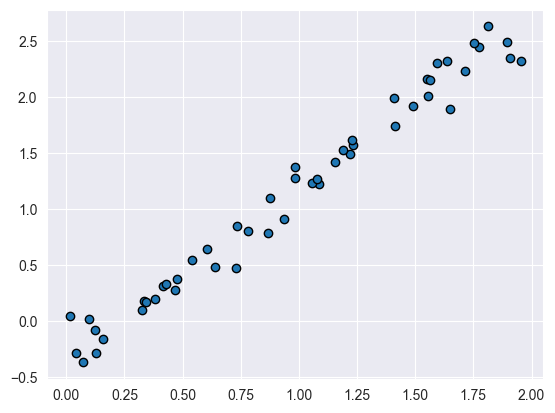
\includegraphics[height=0.3\textheight]{example1.png}

\end{frame}

\section{The procedure}

%%%%
\begin{frame}[fragile]
\frametitle{Finding the LSR line}
\begin{figure}\label{fig:running-example}
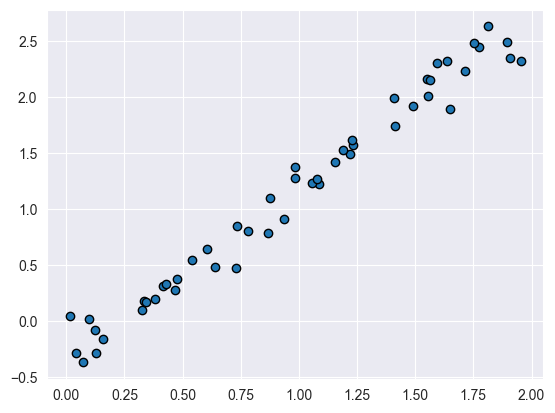
\includegraphics[height=0.4\textheight]{example1.png}
\caption{Our running example}
\end{figure}

\vspace*{-6pt}
How do we find the LSR line?

\pause
NumPy will do this:  if \ct{x}, \ct{y} are the arrays containing the $x$- and $y$-coordinates, the slope and intercept for LSR line are given by:


\begin{codeblock}

\begin{python}[numbers=none]
np.polyfit(x,y,1)
\end{python}

\end{codeblock}

\end{frame}

%%%%
\begin{frame}[fragile]
\frametitle{Finding the LSR line}
% \begin{figure}\label{fig:running-example}
% 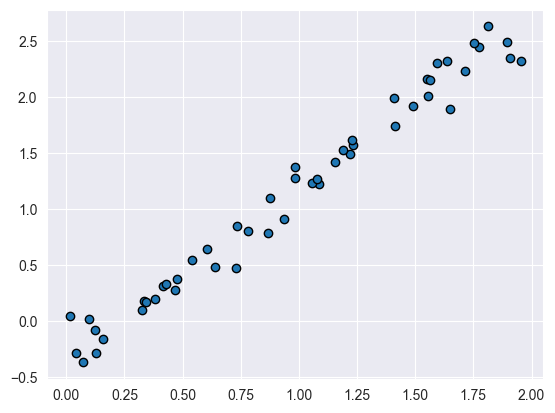
\includegraphics[height=0.3\textheight]{example1.png}
% \caption{Our running example}
% \end{figure}

But, how?  What is procedure to find the slope, intercept?

\pause
\begin{itemize}
    \item If a slope $w$ and intercept $b$ existed so that $(x_1,y_1),\ldots,(x_{50},y_{50})$ \emph{were} points on $y = wx+b$, then 
    \[y_i = wx_i + b\]
would hold for all $1\le i\le 50$.
\end{itemize}

\pause
\begin{enumerate}
    \item Write those 50 equations as a matrix equation. Setting: 
    \[{\scriptsize A = \begin{bmatrix}1 & x_1 \\ 1 & x_2 \\ \vdots & \vdots \\ 1 & x_{50}\end{bmatrix}; \qquad 
      {\bf y} = \begin{bmatrix}y_1 \\ y_2 \\ \vdots \\ y_{50}\end{bmatrix}, }\]
    and writing\footnote{Will use $\tilde{\bf w}$ for this vector, for the rest of these slides.} $\tilde{\bf w} = $ {\small $\begin{bmatrix}b\\ w\end{bmatrix}$}, the matrix equation is $A\tilde{\textbf{w}} = {\bf y}$.
\end{enumerate}
    
\vfill
\end{frame}
    
%%%%
\begin{frame}
\frametitle{Finding the LSR line}
Now the equation $A\tilde{\bf w} = {\bf y}$ does not have a solution (those points are \emph{not} on a line). 

\onslide<2-> 
\textbf{Considering points as approx. on a line:} (\emph{noise in $y$-coordinate direction}) 
\begin{itemize}
    \item Find a $\hat{\bf y}$ \emph{as close to} ${\bf y}$ \emph{as possible} so that $A\tilde{\bf w} = \hat{\bf y}$ has a solution. For each $i$, making a (hopefully small) change $y_i \leadsto \hat{y}_i$ to get $\hat{\bf y}$.
\end{itemize}

\begin{multicols}{2}
\onslide<3->{
\begin{enumerate}
\setcounter{enumi}{1}
    \item Done by solving \mbox{$A^TA\tilde{\bf w} = A^T{\bf y}$ (normal equations).} \newline 
If solution is $\tilde{\bf w}^\star = \begin{bmatrix}b^\star \\ w^\star\end{bmatrix}$, then $\hat{\bf y}=A\tilde{\bf w}^\star$.
\end{enumerate}
}

\onslide<2->{
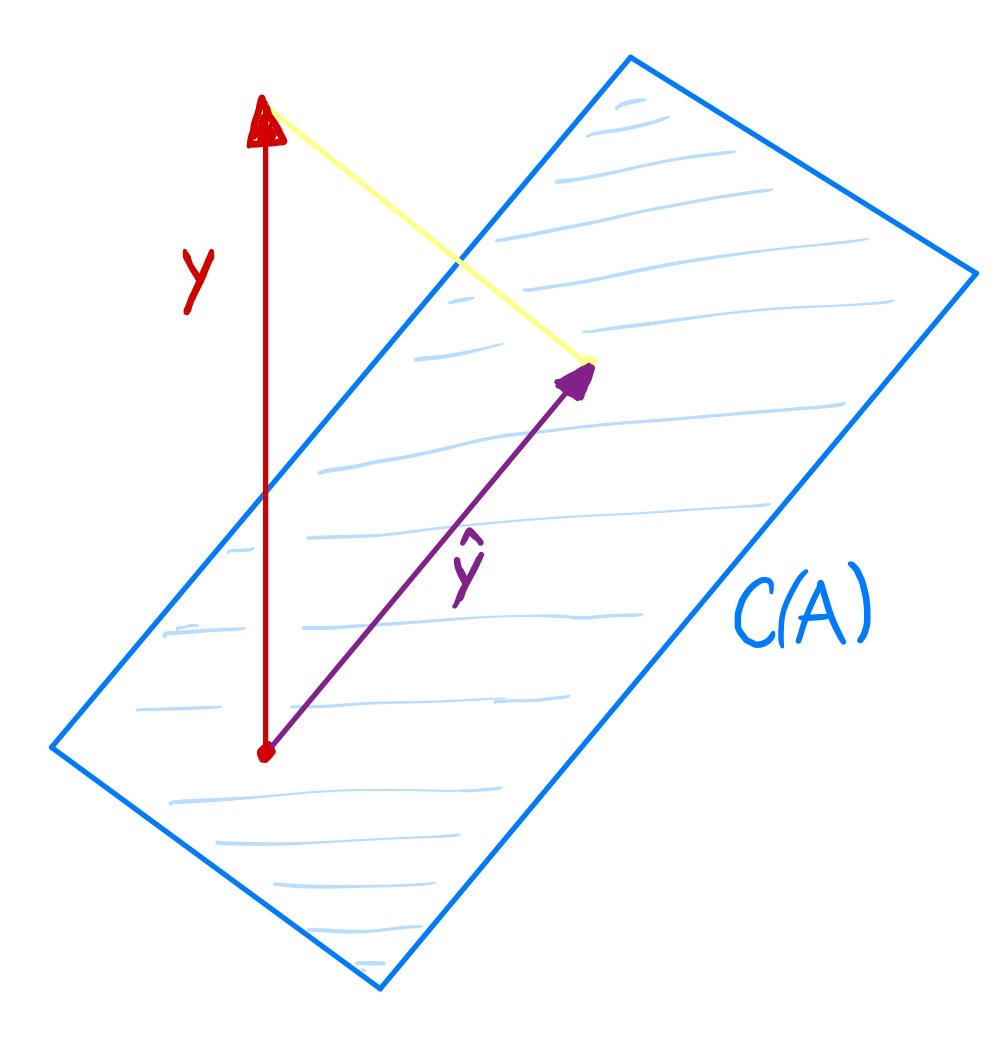
\includegraphics[height=0.3\textheight]{Project_to_CA.jpeg}
}
\end{multicols}

\end{frame}

%%%%
\begin{frame}
\frametitle{Normal equation}
Why does solving $A^TA\tilde{\bf w} = A^T{\bf y}$ give the right thing?
\vspace*{12pt}

\pause
Related to orthogonal vectors in $\mathbb R^P$ (in the example, $\mathbb R^{50}$).

\begin{itemize}
    %\item If $A\tilde{\bf w} = \hat{\bf y}$ has a solution, then $\hat{\bf y}\in\mathbb R^{50}$ is in column space of $A$.
    %\pause
    \item ${\bf y} = {\bf z}_1 + {\bf z}_2$, for some ${\bf z}_1$ in null space of $A^T$,\ ${\bf z}_2$ in column space of $A$.\newline 
    \qquad (\emph{Note: Null space of $A^T$ orthogonal to column space of $A$.})
    \pause
    \item ${\bf z}_2$ is closest to ${\bf y}$ (in col.~space), since ${\bf z}_1$ is orthogonal to column space: ${\bf z}_2 = \hat{\bf y}$. 
    \pause
    \item As ${\bf z}_2$ in column space, $\exists$ $\tilde{\bf w}^\star$ so that $A\tilde{\bf w}^\star = {\bf z}_2 = \hat{\bf y}$.\pause \hspace*{0.5em}
    But then, 
    \[A^T(A\tilde{\bf w}^\star) = A^T{\bf z}_2 = A^T({\bf y} - {\bf z}_1) = A^T{\bf y}.\]
    So the $\tilde{\bf w}^\star$ that you want must be a solution to the normal equations.
\end{itemize}

\end{frame}

%%%%
\begin{frame}
\frametitle{Finding the LSR line}
\textbf{Normal equations:} 
\[(A^TA)\tilde{\bf w} = A^T{\bf y}.\]

\pause
\textbf{Note:}
\begin{itemize}
    \item $A^TA$ is $2\times 2$ matrix, $A^T{\bf y}\in\mathbb R^2$, and $A^TA$ is invertible as long as there exists $x_i\ne x_j$.
\end{itemize}

\pause 
\begin{enumerate}
\setcounter{enumi}{2}
    \item Pretty quick to find solution to $(A^TA)\tilde{\bf w} = A^T{\bf y}$.
\end{enumerate}

\pause 
So, three steps: 
\begin{enumerate}
    \item Write the $P$ equations in matrix form. (get matrix $A$, vector ${\bf y}$)
    \item Get matrix $A^TA$ and vector $A^T{\bf y}$ for normal equations.
    \item Use a method to solve normal equations for $\tilde{\bf w}$.
\end{enumerate}
\end{frame}

\section{Implementing the procedure}

%%%%
\begin{frame}[fragile]
\frametitle{Solving normal equation, in pseudocode}
Procedure to carry out the steps:
\begin{enumerate}
    \item Write the $P$ equations in matrix form. (get matrix $A$, vector ${\bf y}$)
    \item Get matrix $A^TA$ and vector $A^T{\bf y}$ for normal equations.
    \item Use a method to solve normal equations for $\tilde{\bf w}$.
\end{enumerate}

\pause
\vspace*{12pt}
Given $(x_1,y_1), (x_2,y_2), \ldots, (x_P, y_P)$, as a NumPy array (call it \ct{D}, with shape \ct{(P,2)}): 

\begin{pseudo}
A = [ [1, x1], ..., [1, xP] ] # 2-column matrix
y = y-coordinate array
# next, get 2x2 matrix and 2-vector
Compute A.T times A; compute A.T times y
Solve normal eq'ns (e.g., using inverse)
return solution 
\end{pseudo}

\end{frame}

\section{Examples}

%%%%
\begin{frame}
\frametitle{Result on running example}
For the data (linked to above) with 50 points, the LSR line comes out close to
    \[y = 1.520275x - 0.33458.\]
($b^\star = -0.33458$ and $w^\star = 1.520275$)

\pause
A plot of the line (in red), alongside the points, looks as follows.

\vspace*{8pt}
\centering
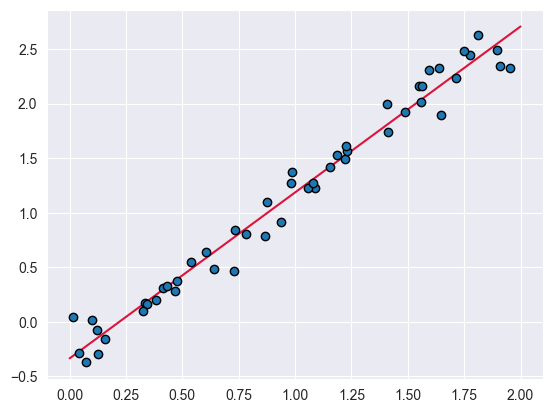
\includegraphics[height=0.4\textheight]{example1-lsrline.png}
\end{frame}

%%%%
\begin{frame}[fragile]
\frametitle{Another example, Advertising data}
In the \href{https://github.com/cornwell/math371-F25/blob/main/DataSets/}{DataSets folder}, the \ct{'Advertising.csv'} file contains data on amounts spent (in thousands of dollars) on TV, Radio, and Newspaper advertising in 200 different markets, as well as the amounts sold in each market (in thousands of units).

\pause
We will look more at this data later. For now, plotted here are the columns \ct{('TV', 'Sales')}.

\vspace*{12pt}
\centering
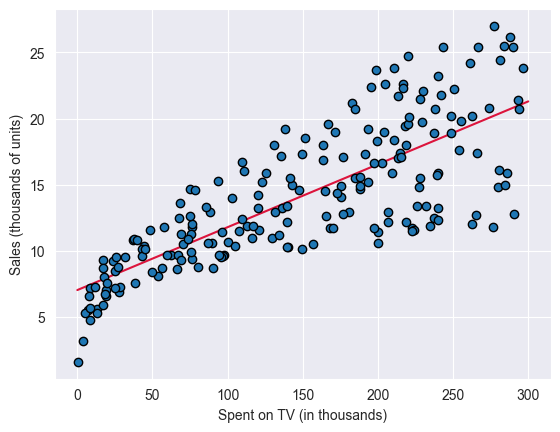
\includegraphics[height=0.4\textheight]{advertising-plot1.png}

\end{frame}

%%%%
\begin{frame}[fragile]
\frametitle{Another example, Advertising data}
If you switch the role of $x$- and $y$-coordinates, you can still do linear regression; \textit{i.e.}, for purpose of a thought experiment, predict the TV data as the \emph{response}, instead of the Sales.

\onslide<2->{
The LSR line for the data is then \textbf{not} the same line, if you switch the roles of TV and Sales in the algorithm to get $\tilde{\bf w}^\star$.
}

\vspace*{3pt}
\centering
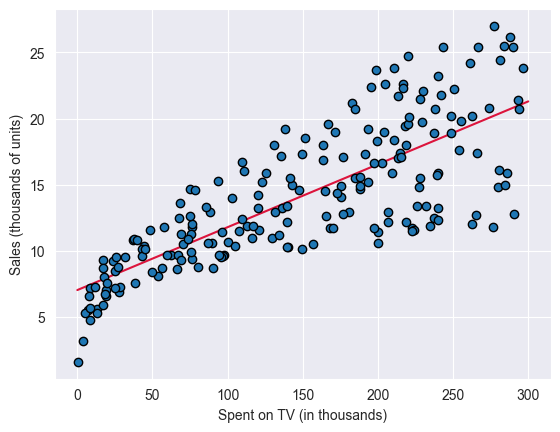
\includegraphics[height=0.4\textheight]{advertising-plot1.png}
\vfill

\end{frame}
    
%%%%
\begin{frame}[fragile]
\frametitle{Another example, Advertising data}
If you switch the role of $x$- and $y$-coordinates, you can still do linear regression; \textit{i.e.}, for purpose of a thought experiment, predict the TV data as the \emph{response}, instead of the Sales.

The LSR line for the data is then \textbf{not} the same line, if you switch the roles of TV and Sales in the algorithm to get $\tilde{\bf w}^\star$. (Use \underline{domain knowledge}.)

\centering
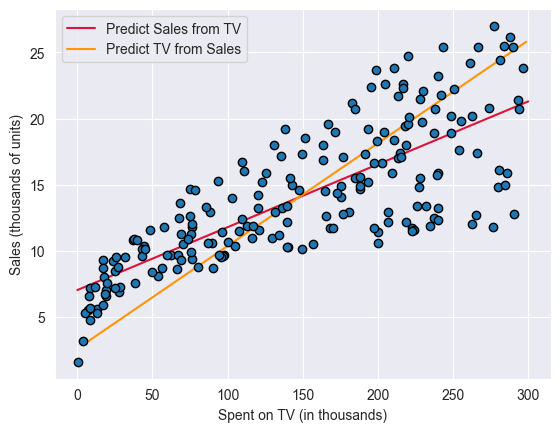
\includegraphics[height=0.4\textheight]{advertising-plot2.png}
\vfill

\end{frame}

\end{document}